\begin{center}
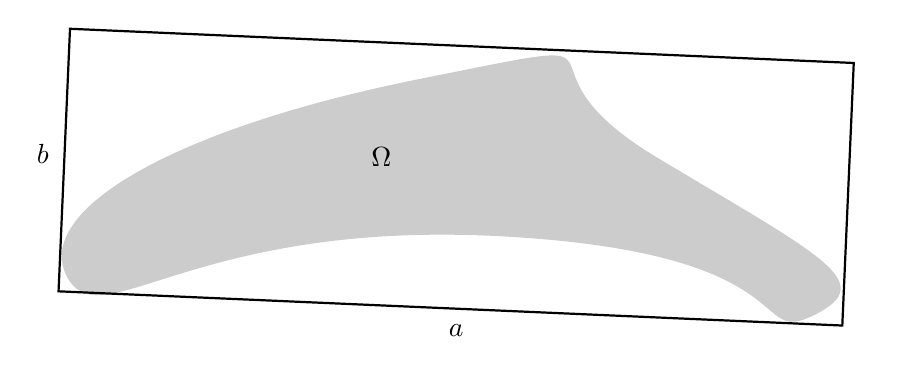
\begin{tikzpicture}[x=1cm,y=1cm]

%omega
\fill[gray!40] plot[smooth cycle,tension=1.5] 
coordinates {
%(1.5,7.2)
(4,2)
%(7,7.1)
(7,1)
%(12,4.2)
%(11.8,2.1)
(9,-1)  % a on bottom
%(8,0.4)
(5,0)
%(2.5,1.8)
(-.5,-.5)
};

%box
\coordinate (BL) at (-0.6,-.7); % Bottom-Left of the *unrotated* box
\coordinate (BR) at (9.5,-.7); % Bottom-Right
\coordinate (TR) at (9.5,2.2);  % Top-Right
\coordinate (TL) at (-0.6,2.2);  % Top-Left

\begin{scope}[rotate around={-2.5:(4.75,0)}] % Rotate the box around the center of G
    \draw[black, thick] (BL) rectangle (TR);

    % Label sides 'a' and 'b' on the rotated box
    % You'll need to adjust positions slightly based on rotation
    \path (BL) -- (BR) node[midway, below=3mm] (label_a) {$a$};
    \path (BL) -- (TL) node[left, pos=0.6] (label_b) {$b$};
\end{scope}

%labels
\node at (3.5,1) {$\Omega$};
\end{tikzpicture}
\end{center}